\documentclass[12 pt, letterpaper]{exam}
\printanswers
\usepackage{amsfonts}
\usepackage{graphicx}
\usepackage{amsthm}
\usepackage{amssymb}
\usepackage{amsmath}
\usepackage{enumerate, mathrsfs}
\usepackage[framed,indented,numbered,autolinebreaks,useliterate]{mcode}


\theoremstyle{definition}
\newtheorem{ex}{Example}
\newtheorem{df}{Definition}
\newtheorem{thm}{Theorem}
\newtheorem{prob}{Problem}

\newcommand{\suchthat}{\,\Big{|}\,}
\newcommand{\ZZ}{\mathbb{Z}}
\newcommand{\QQ}{\mathbb{Q}}
\newcommand{\NN}{\mathbb{N}}
\newcommand{\RR}{\mathbb{R}}
\newcommand{\CC}{\mathbb{C}}
\newcommand{\dd}{\,\,\textrm{d}}

\firstpageheader{Math 3900 Spring 2019}{Homework 3}{Instructor:  J. Haga}
\begin{document}
\begin{questions}
\question Suppose $f(x) = 3^{x}$.  
\begin{parts}
\part[15] Use the data $$f(-1)=\frac{1}{3} \quad \quad f(0) = 1 \quad \quad f(1)=3 \quad \quad f(2)=9$$ to construct a cubic Lagrange interpolating polynomial $P$ for $f$.  Express $P$ in the standard form $P(x) = \frac{a_3}{b_3}x^3 + \frac{a_2}{b_2}x^2 + \frac{a_1}{b_1}x+\frac{a_0}{b_0}$ where $a_i,b_i\in \ZZ$ for $0\leq i\leq 3$.
\begin{solution}
    Our unsimplified solution starts as:
    $$P(x) = \frac{1}{3} \times \frac{(x)(x-1)(x-2)}{(-1)(-1-1)(-1-2)} + 1 \times \frac{(x+1)(x-1)(x-2)}{(1)(0-1)(0-2)} +$$
    $$3 \times \frac{(x+1)(x)(x-2)}{(1+1)(1)(1-2)} + 9 \times \frac{(x+1)(x)(x-1)}{(2+1)(2)(2-1)}$$

    Simplified into stardard form, it looks like:
    $$P(x) = \frac{4}{9}x^3+\frac{2}{3}x^2+\frac{8}{9}x+1$$
\end{solution}
\part[5] Use Desmos to produce a graph of both $f$ and $P$ in the window $-10\leq y\leq 10$, $-5\leq x\leq 5$ (use the Share Graph feature to export a .png of this graph and embed it in your pdf).  Comment qualitatively on the degree to which $P$ fits $f$ on this rectangle.  
\begin{solution}
    It fits well for most of the graph in this rectangle. For $x<-1$ $P$ starts to become a really poor fit for $f$.
    \newpage
    \begin{center}
        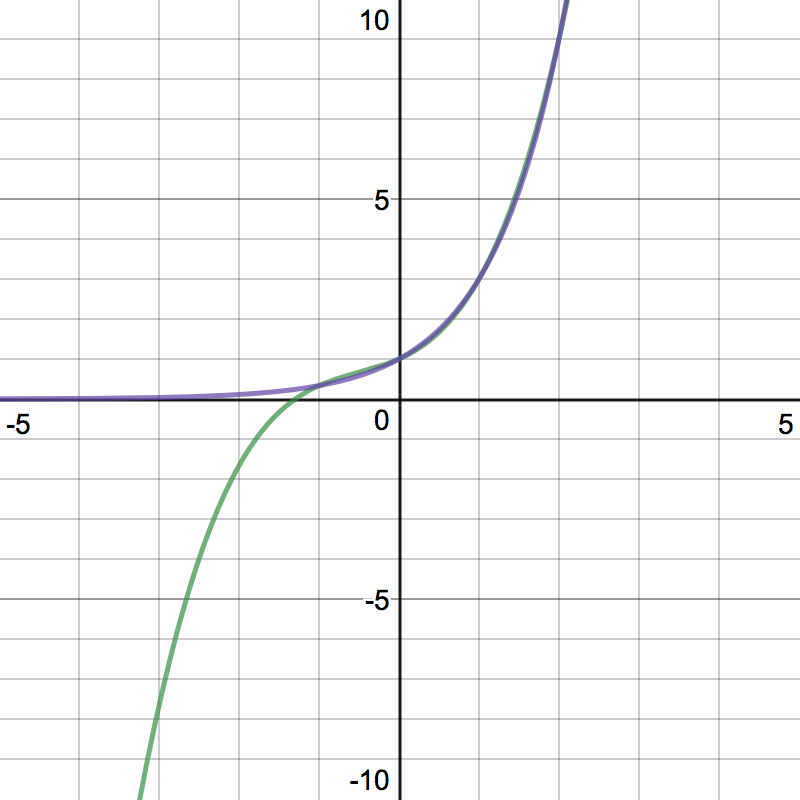
\includegraphics[width=3in]{1b-graph.png}

        (Purple is $f$, Green is $P$)
    \end{center}
\end{solution}
\part[5] Use $P(1/2)$ to determine a rational approximation of $\sqrt 3$; express this approximation as a fraction in lowest terms.
\begin{solution}
    $$P(\frac{1}{2}) = \frac{4}{9} \times (\frac{1}{2})^3+\frac{2}{3} \times (\frac{1}{2})^2+\frac{8}{9} \times \frac{1}{2}+1$$
    $$P(\frac{1}{2}) = \frac{5}{3}$$
\end{solution}
\part[5] Using the single precision representation $\sqrt 3 = 1.73205080756887$, estimate the absolute and relative error in approximating $p=\sqrt 3$ by $p^*=P(1/2)$.
\begin{solution}
    Absolute error:
    $$|p^* - p| = |\frac{5}{3} - 1.73205080756887| = 0.0653841409$$

    Relative error:
    $$\frac{|p^* - p|}{p} = |\frac{0.0653841409}{1.73205080756887}| = 0.03774955135$$
\end{solution}
\part[10] Compare the absolute error from the previous step with the error bound guaranteed by Theorem 3.3.
\begin{solution}
    Theorem 3.3 guarantees that the remainder term will be
    $$\frac{f^{n+1}(\xi(x))}{(n+1)!}(x-x_0)(x-x_1)\cdots(x-x_n)$$
    Given that our $n$ is 3 and $x$ is $\frac{1}{2}$, we can plug in all of our x values and n:
    $$\frac{f^{4}(\xi(\frac{1}{2}))}{(4)!}(\frac{1}{2}+1)(\frac{1}{2})(\frac{1}{2}-1)(\frac{1}{2}-2)$$
    The fourth derivative of $3^x$ is $ln^4(3) \times 3^x$. Knowing this, we can bound $f^{4}(\xi(\frac{1}{2})$ by $f^4(2)$, because $f^4(x)$ is an increasing function. Therefore, we get
    $$\frac{ln^4(4)\times3^2}{24}(0.5625),$$
    which means that our remainder is guaranteed to be bounded by 0.3073 by Theorem 3.3.

    Our absolute error above agrees with that, as it is less than 0.3073.
\end{solution}
\end{parts}

\question Suppose that $f(x) = \sqrt{4-x^2}$.
\begin{parts}
\part[10] Express the Lagrange interpolating polynomial $P(x)$ for $f(x)$ using $x_0=-2$, $x_1=y$, and $x_2=2$, where $y\in (-2,2)$, in the standard form $$P(x) = a_0+a_1x+\cdots+a_kx^k$$  (for the appropriate choice of $k$).  (Your answer will involve the variable $y$).   
\begin{solution}
    We begin by finding the $y$ values of these points, not to be confused with the $y$ variable above: 
    $$f(x_0)=0,\,f(x_1)=\sqrt{4-y^2},\,f(x_2)=0$$
    Now lets list the points:
    $$(-2,0),\,(y,\sqrt{4-y^2}),\,(2,0)$$
    Now time to write out the LIP, notice how two terms of the sum cancel to 0:
    $$P(x)=(\sqrt{4-y^2})\frac{(x+2)(x-2)}{(y+2)(y-2)}$$
    \newpage
    And lets simplify:
    $$P(x)=\frac{(\sqrt{4-y^2})(x^2-4)}{(y^2-4)}$$
    $$P(x)=\frac{(\sqrt{4-y^2})(x^2-4)}{(-1)(4-y^2)}$$
    $$P(x)=\frac{(-1)(\sqrt{4-y^2})(x^2-4)}{(\sqrt{4-y^2})(\sqrt{4-y^2})}$$
    $$P(x)=\frac{(-1)(x^2-4)}{\sqrt{4-y^2}}$$
    $$P(x)=\frac{-x^2+4}{\sqrt{4-y^2}}$$
    $$P(x)=\frac{-x^2}{\sqrt{4-y^2}}+\frac{4}{\sqrt{4-y^2}}$$
\end{solution}
\part[10] Find the largest value of $y\in (-2,2)$ for which $P(0)-f(0)=0.25$.
\begin{solution}
    Lets start by getting $f(0)$ and $P(0)$.
    $$f(0)=2$$
    $$P(0)=\frac{4}{\sqrt{4-y^2}}$$
    Now lets plug into the function:
    $$\frac{4}{\sqrt{4-y^2}}-2=\frac{1}{4}$$
    $$\frac{4}{\sqrt{4-y^2}}=\frac{9}{4}$$
    $$\frac{16}{9}=\sqrt{4-y^2}$$
    $$(\frac{16}{9})^2=4-y^2$$
    $$y^2=4-(\frac{16}{9})^2$$
    $$y=^+_-\sqrt{4-(\frac{16}{9})^2}$$
    We just want the largest $y$ so we take the positive value:
    $$y=\sqrt{\frac{68}{81}}$$
    $$y\approx0.9162$$
\end{solution}
\end{parts}

\question Let $f(x)=|x|$.  Suppose that $P(x)$ is the quintic Lagrange interpolating polynomial for $f$ determined using the points $$(-1,1), (-0.15,0.15), (-0.005,0.005), (0.005,0.005), (0.15,0.15), (1,1).$$
\begin{parts}
\begin{lstlisting}
    function output = neville(x, y, z)
    %{
        Inputs: 
            x: array of x coords
            y: array of y coords
            z: point to evaluate
        Outputs:
            output: the final value from nevilles
    %}
    n = length(x);
    p = zeros(n, n);
    
    for i = 1:n
        p(i, 1) = y(i);
    end
    
    for i=2:n
        for j=2:i
            p(i,j) = (((z-x(i-j+1)) * p(i, j-1)) - ((z-x(i)) * p(i-1, j-1))) / (x(i) - x(i-j+1));
        end
    end
    
    output = p(n, n);
       
\end{lstlisting}
\part[10] Write/execute a MATLAB script that utilizes Neville's method to evaluate $P(0.014)$.

\newpage

\begin{solution}
    Using the matlab script above, we get the output:
\begin{lstlisting}
>> syms f(n);
>> f(n) = abs(n);
>> x = [-1.0000; -0.1500; -0.0050; 0.0050; 0.1500; 1.0000];
>> y = f(x);

>> neville(x, y, 0.014)

ans =

    0.0061
\end{lstlisting}
    Thus, $P(0.014)$ is 0.0061
\end{solution}
\part[5] Determine the absolute and relative errors in using $P(0.015)$ to approximate $f(0.014)$.
\begin{solution}
\begin{lstlisting}
>> neville(x, y, 0.015)

ans =

    0.0063

>> double(abs(neville(x, y, 0.015) - f(0.014)))

ans =

    0.0077

>> double(abs((neville(x, y, 0.015) - f(0.014)) / f(0.014)))

ans =

    0.5489
\end{lstlisting}
\newpage
The absolute error in using $P(0.015)$ to approximate $f(0.014)$ is 0.0077.

The relative error in using $P(0.015)$ to approximate $f(0.014)$ is 0.5489.
\end{solution}

\newpage

\part[10] Write/execute a MATLAB script that utilizes Neville's method to evaluate $P(0.75)$.
\begin{solution}
\begin{lstlisting}
>> neville(x, y, 0.75)

ans =

    1.9384
\end{lstlisting}
$P(0.75) = 1.9384$
\end{solution}
\part[5] Determine the absolute and relative errors in using $P(0.75)$ to approximate $f(0.75)$.
\begin{solution}
\begin{lstlisting}
>> double(abs(neville(x, y, 0.75) - f(0.75)))

ans =

    1.1884

>> double(abs((neville(x, y, 0.75) - f(0.75)) / f(0.75)))

ans =
    
    1.5845
\end{lstlisting}
The absolute error in using $P(0.75)$ to approximate $f(0.75)$ is 1.1884.

The relative error in using $P(0.75)$ to approximate $f(0.75)$ is 1.5845.
\end{solution}
\part[10] Why is it that we cannot use Theorem 3.3 to estimate the error in approximating $f$ by $P$ on $[-1,1]$?
\begin{solution}
We cannot use Theorem 3.3 to estimate the error in $f$ by $P$ because $f$, which is $|x|$, is not differentiable on the closed interveral from -1 to 1.
\end{solution}
\end{parts}
\end{questions}
\end{document}
